\tikzstyle{input_neuron}=[circle,draw=red!50,fill=red!10,thick,minimum size=6mm]
\tikzstyle{hidden_neuron}=[circle,draw=blue!50,fill=cyan!10,thick,minimum size=6mm]
\tikzstyle{output_neuron}=[circle,draw=green!50,fill=green!10,thick,minimum size=6mm]

\tikzstyle{input}=[circle,draw=black!50,fill=black!20,thick,minimum size=6mm]

\begin{center}
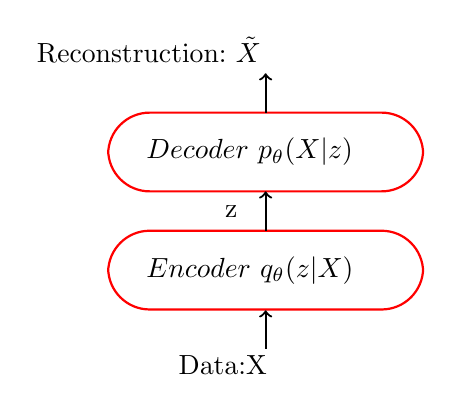
\begin{tikzpicture}

% text
\node[text width=0.007cm] at (7.99,5.25) {z};
\node[text width=0.007cm] at (7.4,3.3) {Data:X};
\node[text width=0.01cm] at (5.6,7.3) {Reconstruction:$\ \tilde{X}$};
\node[text width=0.01cm] at (6.99,4.5){$Encoder\ q_\theta(z|X)$};
\node[text width=0.01cm] at (6.99,6){$Decoder\ p_\theta(X|z)$};

%circular rectangle
\draw[red!100,thick,solid,rounded corners=15pt] (6.5,4) rectangle (10.5,5);
\draw[red!100,thick,solid,rounded corners=15pt] (6.5,5.5) rectangle (10.5,6.5);


%lines
\draw[thick,->] (8.5,3.5) -- (8.5,3.99);

\draw[thick,->] (8.5,5) -- (8.5,5.5);

\draw[thick,->] (8.5,6.5) -- (8.5,7);



\end{tikzpicture}
\end{center}
